\section{ SR0018CA23 }


\subsection{Meta}

    \textbf{Title:}
    Healthcare Operations Research and Management under Pandemics: a Review

    \begin{table}[H]
        \centering
        \begin{tabular}{|c|c|c|c|c|c|c|c|c|}
            \hline
                \textbf{Rank} & \textbf{Grasp} & \textbf{Grade} & \textbf{Type} & \textbf{Outcome} & \textbf{Domain} & \textbf{COV19} & \textbf{CoI} & \textbf{DB} \\
            \hline
                3 & 60\% & B & A & P & B & Yes & Yes & No \\
            \hline
        \end{tabular}
        \caption{Reference's metadata}
        \label{tab:SR0018CA23}
    \end{table}

\subsection{Summary}
    Majid Salavati-Khoshghalb, Masoumeh Kazemi Zanjani, and Nadia Bhuiyan \cite{x128} conducted a preview study on the healthcare OR\&M under a pandemic and collected all related papers in one research. The authors introduced the main methods of predicting and reacting to pandemic outbreaks. This literature review contains a list of studies on medical resource allocation under pandemic pressure. The discussions and further research are unrelated to the medical resource planning and scheduling field and thus have little value to research in resource allocation. Nevertheless, this literature review is an excellent source of inspiration for healthcare professionals working on infections and viruses. Additionally, the work is crucial for policymakers to ensure efficient preparedness and reaction to future pandemic challenges.

\subsection{Notes}
    \begin{itemize}
        \item Has a list of papers about medical resource allocation under pandemic pressure.
    \end{itemize}


\subsection{Reading}
    \textbf{Abstract:}
    This literature review focuses on Operations Research and Management during pandemic overloads of the hospitals' capacities. The authors want to research the effect of crucial desicions in critical times. The World Health Organization categorize the desicions onto two types: preparedness and response. The incterconnections and conflicts amoung different objectives was analysed to better understand the ways of reduce pandemic distructive effects in states and national-wide. 
    
    \textbf{Objectives:}
    The aim is to increase of social welfare from Healthcare System's point of view and public policymakers. 

    
    \textbf{Pages 1-2 (Introduction):}
    History of the worldwide pandemics starting from 1918 to nowadays. Preparedness techniques: tracing the infection disease by monitoring ill population symptoms. The authors will look into desicion making strategies in the next sections. At the end of the section the possible consequences from the pandemic and the structure of the review paper are introduces. 
    \begin{figure}[H]
        \centering
        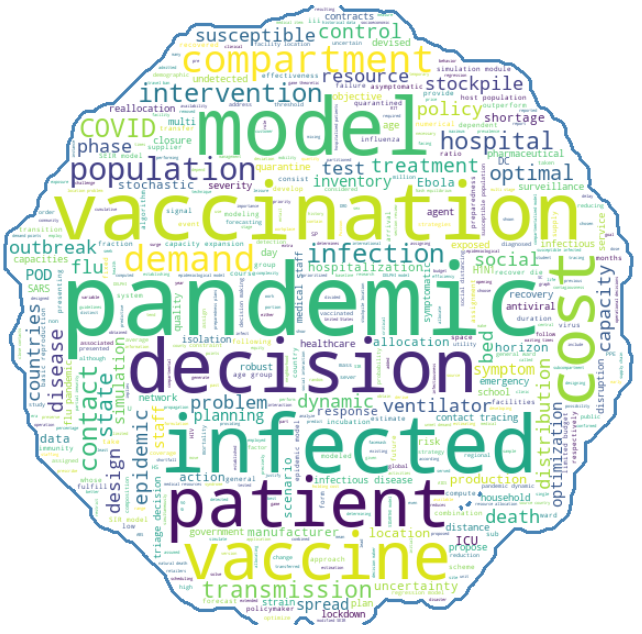
\includegraphics[width=.6\textwidth]{figures/SR0018CA23/fig1.png}
        \caption{Keywords cloud from \cite{x128}.}
        \label{fig1:SR0018CA23}
    \end{figure}
    
    \textbf{Pages 2 (Remark 1):}
    It is not a comparison work it is rather qualitative analysis of the existing knowledge about obsticles, challenges, and solutions to them availbale in the scientific literature.
    
    \textbf{Pages 2-3 (Epidemic Models):}
    The introduction to imitative models for forcasting infection spread and estimate required medical resources. \underline{Compartment models}: population is slit into distinct conmartments and the progress of the pandemic is trecked. The size of compartment is assigned by differential and integral equations. \underline{Network models}: nodes are individual and edges are connections with weights representing probability of these connections. In the compartment model all individuals are the same when connections in network model make the individuals unique entities of the model.

    \textbf{Pages 3-4 (The Compartmentalized Models: SIR, SEIR, and Teir Variants):} 
    This section shows developed compartmentalized models and classification approaches of patients depending on different stages of the infection and other charateristics. The admission policies to PACU and other operational capacieties are discusseda as well.

    \textbf{Pages 4-5 (Network Models):} 
    This section is explained in scope of Agent-Based Simulation (ABS). The section show research cases of simulating the pandemic outpreack scenarios to see how the daily interatctions, activities are influacing the spread of the vidus and how the virus may influance the change in activitis. The individual-to-individual interaction is a key consept for investigation by ABS.
    
    \textbf{Pages 5 (Advance Pandemic Models):}
    Here are presented hybridized models from Compartmentalized and Network models. 
    
    \textbf{Pages 5-6 (Preparedness Plans):}
    Introduction of categories such as syndromic surveillance and contact tracing, stockpile location problem, vaccine composition and production plannig. \underline{Syndromic Surveillance}: the monitoring of population to predict and prevent a possible pandemic outbreak. \underline{Statistical Methods To Declare A Pandemic}: the continiuity for the previous approach.\underline{Previous Experiences to Combat New Epidemics}: Examples of successful implementation of policies of social distancing and vaccination during the COVID-19 crisi.
    
    ...
    
    
    \textbf{Pages 13 (The Allocation of Medical Resources and Personnel):}
    During the pandemic outbreaks the hospitals in the region/ city should work as a single organism for allocating medical resources. In the next sections, the overview how previous pandemics influance the resource allocation problems.
    
    \textbf{Pages 13-14 (Ventilator Allocation):}
    A computer simulation model. A stochastic multi-period suply chain model... and the section continues with summary of other studies without additional analysis from the authors of this review.

    \textbf{Pages 14-15 (Hospital Bed Allocation, Capacity Estimation, Expansions)}... 